\thispagestyle{empty}

\begin{center}
  Федеральное государственное бюджетное образовательное учреждение высшего профессионального образования \\
  <<Костромской государственный университет имени Н. А. Некрасова>> \\
  \vspace{1em}
  Кафедра теории и истории культур
\end{center}
\vspace{.1em}
\begin{flushright}
  \textit{На правах рукописи} \\
  \vspace{14pt}
  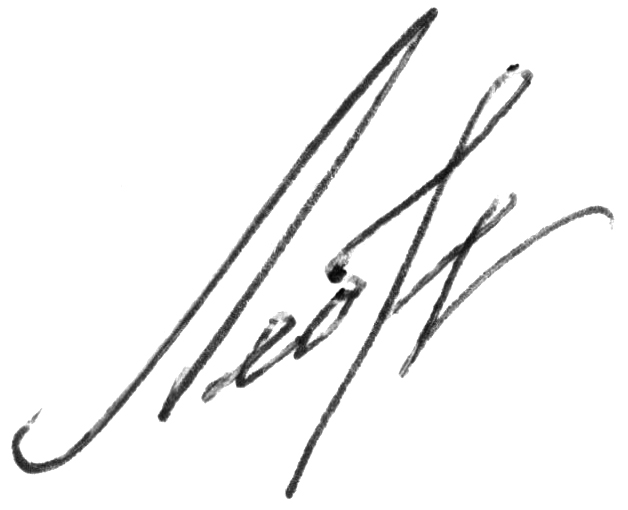
\includegraphics[width=2.9cm]{images/lebedev}
\end{flushright}
\begin{center}
  \textbf{ЛЕБЕДЕВ Никита Андреевич} \\
  \vspace{3em}
  \textbf{ЛОГОТИП КАК ФОРМА МАССОВОГО СОЗНАНИЯ:\\
    СТРУКТУРА, ФУНКЦИИ, ЭМБЛЕМАТИКА} \\
  \vspace{3em}
  Специальность 24.00.01 – теория и история культуры \\
  \vspace{3em}
  \textbf{Диссертация} \\
  на соискание ученой степени \\
  кандидата культурологии
\end{center}
\vspace{3em}
\begin{flushright}
  Научный руководитель: \\
  доктор культурологии, \\
  профессор И. А. Едошина
\end{flushright}

\vspace{6em}
\begin{center}
  Кострома 2013
\end{center}
